%%%%%%%%%%%%%%%%%%%%%%%%%%%%%%%%%%%%%%%%%%%%%%%%%%%%%%%%%%%%%%%%%%%%%
% LaTeX Template: Project Titlepage Modified (v 0.1) by rcx
%
% Original Source: http://www.howtotex.com
% Date: February 2014
% 
% This is a title page template which be used for articles & reports.
% 
% This is the modified version of the original Latex template from
% aforementioned website.
% 
%%%%%%%%%%%%%%%%%%%%%%%%%%%%%%%%%%%%%%%%%%%%%%%%%%%%%%%%%%%%%%%%%%%%%%

\documentclass[12pt]{report}
\usepackage[a4paper]{geometry}
\usepackage[myheadings]{fullpage}
\usepackage{fancyhdr}
\usepackage{lastpage}
\usepackage{graphicx, wrapfig, subcaption, setspace, booktabs}
\usepackage[T1]{fontenc}
\usepackage[font=small, labelfont=bf]{caption}
\usepackage{fourier}
\usepackage[protrusion=true, expansion=true]{microtype}
\usepackage[english]{babel}
\usepackage{sectsty}
\usepackage{url, lipsum}
\usepackage{natbib}
% \usepackage{biblatex}
\newcommand{\HRule}[1]{\rule{\linewidth}{#1}}
\onehalfspacing
\setcounter{tocdepth}{5}
\setcounter{secnumdepth}{5}
\usepackage{graphicx}
\usepackage{xcolor}
\usepackage{hyperref}
\protected\def\mycolor{\color{red}}
%-------------------------------------------------------------------------------
% HEADER & FOOTER
%-------------------------------------------------------------------------------
\pagestyle{fancy}
\fancyhf{}
\setlength\headheight{15pt}
\fancyhead[L]{BE PROJECT}
\fancyhead[R]{LITERATURE SURVEY}
\fancyfoot[R]{Page \thepage\ of \pageref{LastPage}}
%-------------------------------------------------------------------------------
% TITLE PAGE
%-------------------------------------------------------------------------------
\newcommand{\todolink}[1]{\noindent{\color{blue}\href{#1}{#1}}}
\newcommand{\todo}[1]{\noindent{\color{red}#1}}
\newcommand{\edit}[1]{{\color{blue}#1}}
\newcommand{\refsec}[1]{Section~\ref{#1}}
\newcommand{\reffig}[1]{\mbox{Figure~\ref{#1}}}
\newcommand{\reftab}[1]{Table~\ref{#1}}
\newcommand{\refeq}[1]{Eq.~\ref{#1}}
\newcommand{\etal}{~et~al.}
\newcommand{\ttt}[1]{{\small \texttt{#1}}}

\begin{document}

\title{ \normalsize \textsc{}
		\\ [2.0cm]
		\HRule{0.5pt} \\
		\LARGE \textbf{\uppercase{Serverless Computing?}}
		\HRule{2pt} \\ [0.5cm]
		\normalsize  \vspace*{5\baselineskip}}

\date{}

\author{
        Jerad Hoy \\
        Saidur Rahman \\ 
        Montana State University}
        
\newpage
\maketitle

%-------------------------------------------------------------------------------
% Section title formatting
% \sectionfont{\scshape}
%-------------------------------------------------------------------------------

%-------------------------------------------------------------------------------
% BODY

\section*{Introduction}
\label{sec:introduction}
%what is serverless?

Nowadays, Serverless Computing is becoming a popular technology.  It is a system that provides backend services on an as-used basis.
It also provides users to write and deploy code without worrying about the underlying support. It also handles all the system administration operations to make programmers' life more comfortable. If users use serverless technology for backend services, the user needs to pay based on their usage. They do not need to pay a fixed amount of bandwidth or number of servers because the service is autoscaling \cite{shafiei2019serverless,wu2020}. Note that though the name is serverless, physical servers are still needed, but the developers do not need to be aware of it. \reffig{fig:serverless} shows the transformation of services from physical machines to Serverless.

\begin{figure}[!ht]
	\centering
	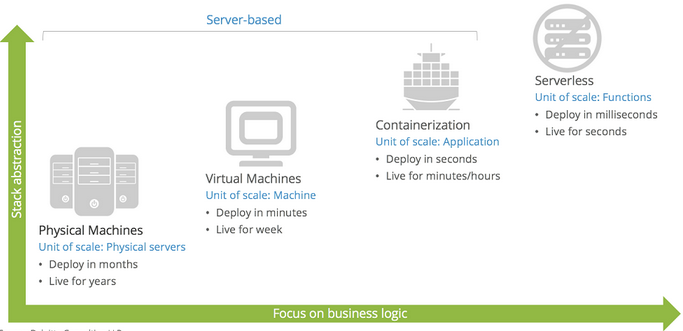
\includegraphics[width=1.0\textwidth]{images/serverless.png}
	\caption{Road to Serverless (\todo{redraw:https://deloitte.wsj.com/cio/2017/11/09/serverless-computings-many-potential-benefits/})}
	\centering
	\label{fig:serverless}
\end{figure}

%how it works?

% types of server-less

%why is better than other system?


\todo{list of papers:}\\
\todolink{https://www.sciencedirect.com/science/article/pii/S0167739X17316485}\\
\todolink{https://www2.eecs.berkeley.edu/Pubs/TechRpts/2019/EECS-2019-3.pdf}\\
\todolink{https://www.cloudflare.com/learning/serverless/why-use-serverless/}\\
\todolink{https://ieeexplore.ieee.org/document/9183650}\\
\todolink{https://assets.amazon.science/96/c6/302e527240a3b1f86c86c3e8fc3d/firecracker-lightweight-virtualization-for-serverless-applications.pdf}\\
\todolink{https://ieeexplore.ieee.org/document/8457830}\\
\todolink{https://ieeexplore.ieee.org/document/8605774}\\
\todolink{https://ieeexplore.ieee.org/document/9213020}\\
\todolink{https://ieeexplore.ieee.org/document/9058237}\\
\todolink{https://ieeexplore.ieee.org/document/9213030}\\
\todolink{https://ieeexplore.ieee.org/document/7979854}\\
\todolink{https://ieeexplore.ieee.org/document/9213030}\\
\todolink{https://www.computer.org/csdl/magazine/so/5555/01/09214403/1nHNGfu2Ypi}\\
\todolink{https://cacm.acm.org/magazines/2019/12/241054-the-rise-of-serverless-computing/fulltext}\\
\todolink{https://www.singlemindconsulting.com/blog/server-vs-serverless-a-performance-test/}\\
\todolink{https://ieeexplore.ieee.org/abstract/document/9180214}\\
\todolink{https://ieeexplore.ieee.org/document/969727}\\
\todolink{https://dl.acm.org/doi/10.1145/3276488}\\
\todolink{https://www.serverless.com/blog/serverless-faas-vs-containers}
\section*{Related Work}
\label{sec:related_work}
% \todo{Saidur will work on it}\\

The perspective of serverless applications requires multiple clients' workload run on the same hardware with minimal overhead. However, the container provides weak security and minimal overhead, where the virtualization provides robust security and high overhead. So, Alexandru \etal\ developed Firecracker, a new open-source Virtual Machine Monitor (VMM) specialized for serverless workloads but generally useful for containers, functions, and other compute workloads within a reasonable set of constraints \cite{firecracker}.


Serverless services impose severe restrictions for some applications, such as using a predefined set of programming languages or difficulty installing and deploying external libraries. The author \cite{PEREZ201850} proposed a framework and a methodology to create Serverless Container-aware ARchitectures (SCAR). The SCAR framework creates highly-parallel event-driven serverless applications that run on customized runtime environments.

Hyungro \etal\ hypothesizes that the current serverless computing environments can support dynamic applications parallel when a partitioned task is executable on a small function instance. To verify the hypothesis, they deployed a series of functions for distributed data processing to address the elasticity and then demonstrated the differences between serverless computing and virtual machines for cost efficiency and resource utilization based on throughput, network bandwidth, a file I/O \cite{lee2018performance}. 

Serverless FaaS Functions are triggered by users and are provisioned dynamically through containers or virtual machines(VMs). However, the start-up delays of containers or VMs usually lead to the relatively high latency of response to cloud users. Moreover, the communication between different functions generally depends on virtual net devices or shared memory and may cause extremely high-performance overhead. The authors \cite{tan2020unikernel} propose a lightweight approach to serverless computing named Unikernel-as-a-Function(UaaF) that offers extremely low start-up latency to execute functions and an efficient communication model to speed up inter-functions interactions. They also employ a new hardware technique VMFUNC to invoke functions in other unikernels seamlessly like IPC.


Linux containers offer a lightweight service to load applications into images, put them in isolated environments, and scan periodically to detect vulnerabilities using a vulnerability scanning service. The authors \cite{bila2017serverless} investigate the same architecture for mitigating the threat to a serverless architecture.


Kalev \etal\ shows a method named Trapeze to provide security on serverless systems using dynamic information flow control (IFC). It encapsulates each serverless function in a sandbox, redirecting all the interactions to the security shim and enforces the global security policy~\cite{alpernas2018}. 

% \subsection*{Container}
% \subsection*{VM}
% \subsection*{Serverless Computing}

\section*{Serverless Architecture \& Performance Evaluation}

% % \todo{Jerad will work on it}\\
% Nowadays, Linux workloads can be categorized into three parts: containers, virtualization, and language VM isolation.

% Here is the general view of serverless architecture shown in \reffig{fig:arc_serverless}. When a invoke occurs, frontend Invoke REST API gets the request and check for authorization and load the function metadata. 

% \todo{Jerad: please complete the rest of the part: check section: 4.1.1}

% \todolink{https://assets.amazon.science/96/c6/302e527240a3b1f86c86c3e8fc3d/firecracker-lightweight-virtualization-for-serverless-applications.pdf}

% \begin{figure}[!ht]
% 	\centering
% 	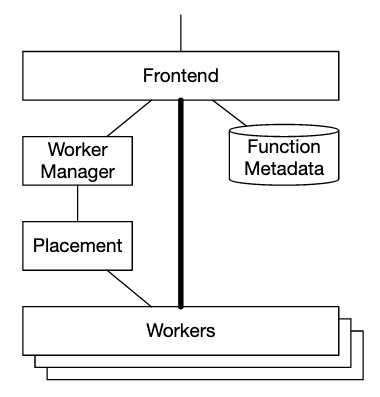
\includegraphics[width=0.5\textwidth]{images/serverless_architecture.png}
% 	\caption{Serverless Worker-Manager architecture \cite{firecracker}}
% 	\centering
% 	\label{fig:arc_serverless}
% \end{figure}


\label{sec:solution}
\subsection*{SCAR: Serverless Computing for Container-based Architectures}
This paper proposed a methodology to create Serverless Container-aware ARchitectures (SCAR) \cite{PEREZ201850} to solve the installation and deployment of external libraries that are not predefined. The SCAR can be used to serve event-driven and highly-parallel serverless applications that run on customized runtime environments defined as Docker images on top of AWS Lambda. \reffig{fig:scar_architecture} shows the architecture of SCAR. SCAR enables users to assign Lambda functions. When an invocation occurs, a container from the Docker image, which is stored in a Docker hub, will be executed. The architecture has two sections: SCAR client and SCAR server. SCAR Client is a python script to validate input, create the deployment including udocker, create the Lambda function with SCAR supervisor, manage the configuration to trigger events from S3~\cite{s3} to Lambda. SCAR server represents the Lambda function's code (Python 3.6) and retrieves the Docker image using udocker from Docker hub. First, the user selects a Docker image available in Docker Hub and generates the Lambda with the user's configuration. The user can directly invoke the Lambda function where the SCAR supervisor is triggered, which is ended up executing a container out of a Docker image and optionally run a user-defined shell script. Data staging from and to S3 is automatically managed by the SCAR supervisor and diverted the logs into CloudWatch.
\begin{figure}[!t]
	\centering
	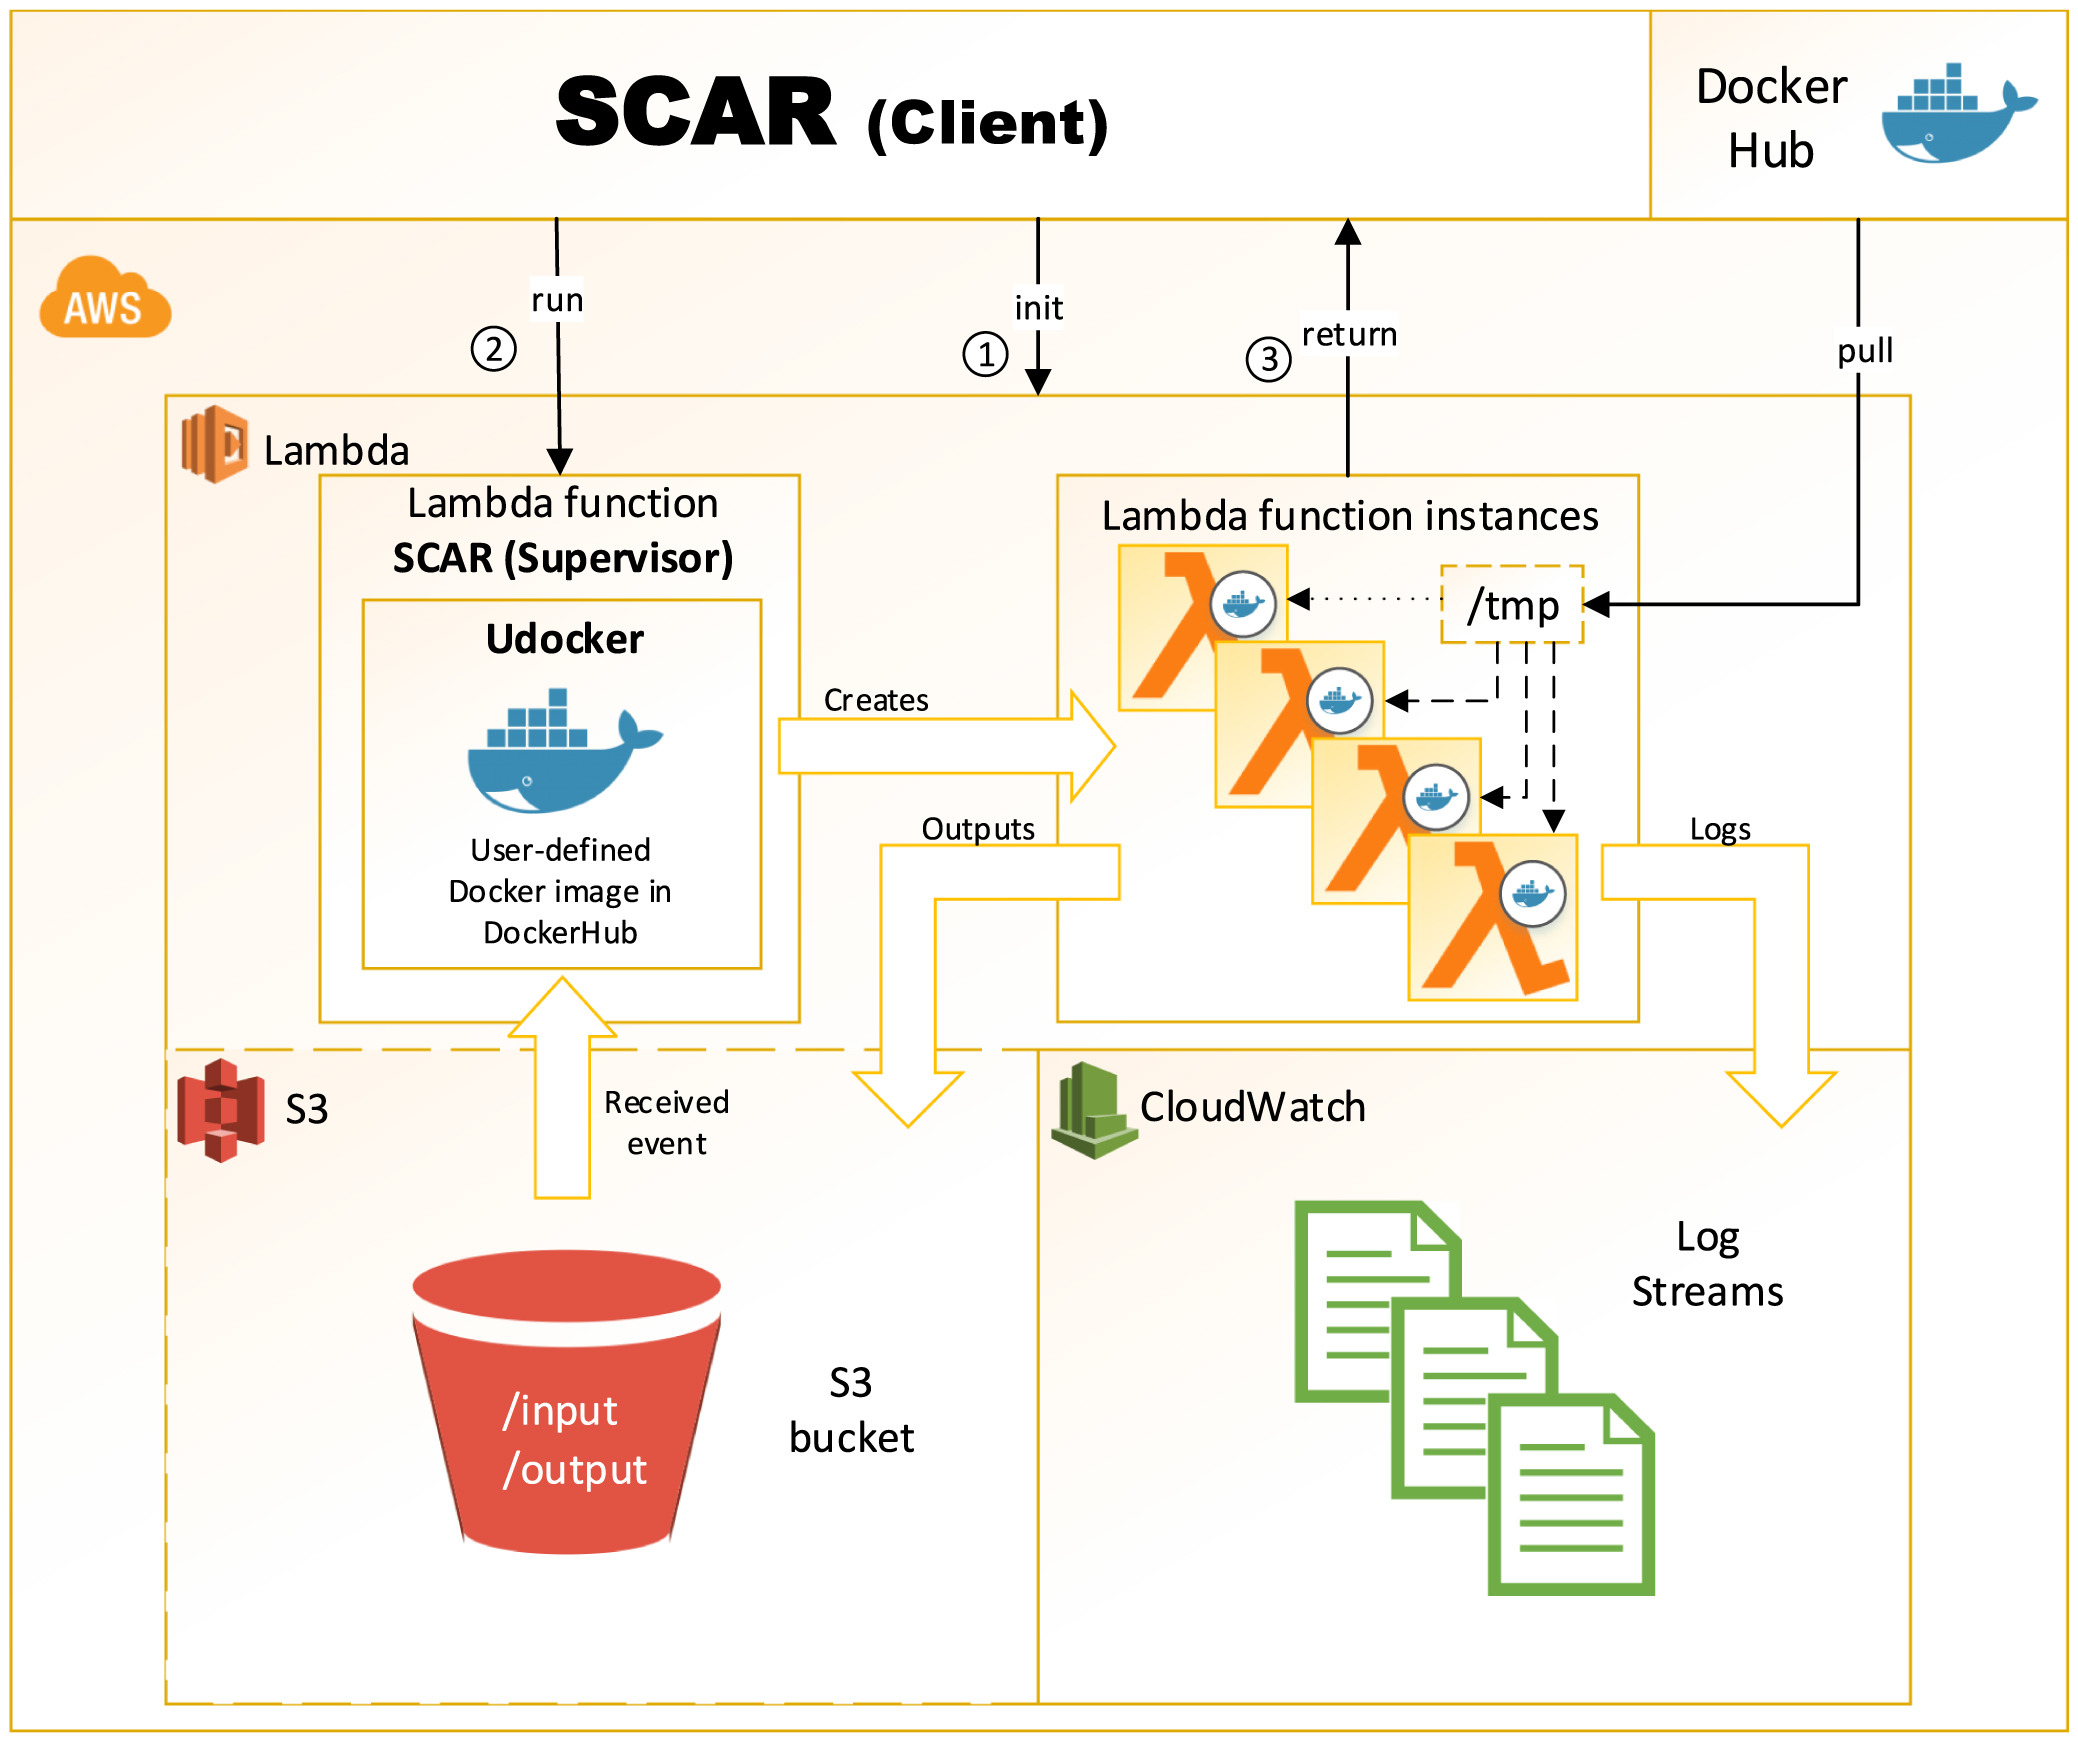
\includegraphics[width=0.7\textwidth]{images/scar_architecture.jpg}
	\caption{SCAR Architecture \cite{PEREZ201850}}
	\centering
	\label{fig:scar_architecture}
\end{figure}

\begin{figure*}[!b]
\centering % <-- added
\begin{subfigure}{0.32\textwidth}
  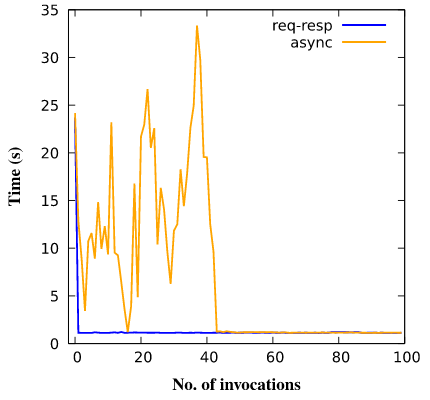
\includegraphics[width=\linewidth]{images/scar-1.png}
  \caption{Average execution time(in seconds) for each invocation type \cite{PEREZ201850}}
  \label{fig:scar1}
\end{subfigure} \hfil% <-- added
\begin{subfigure}{0.33\textwidth}
  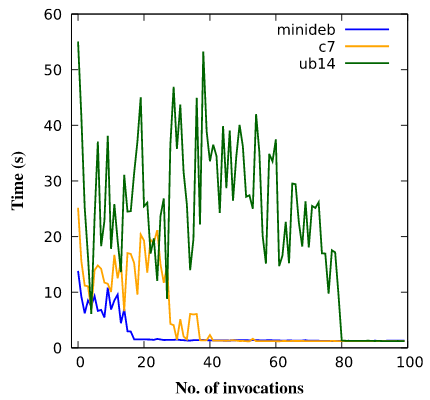
\includegraphics[width=\linewidth]{images/scar-3.png}
  \caption{Average execution time (in seconds) for different container sizes (all synchronous) \cite{PEREZ201850}}
  \label{fig:scar3}
\end{subfigure} \hfil% <-- added
\begin{subfigure}{0.33\textwidth}
  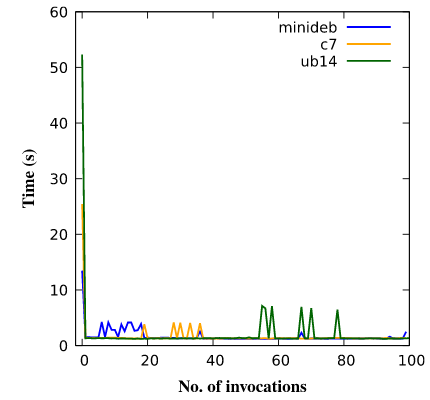
\includegraphics[width=\linewidth]{images/scar-4.png}
  \caption{Average execution time (in seconds) for different container sizes (First invocation req-res and subsequent are asynchronous) \cite{PEREZ201850}}
  \label{fig:scar4}
\end{subfigure} \hfil% <-- added
\caption{SCAR Performance}
\label{fig:scar_performance}
\end{figure*}
% \begin{itemize}
%     \item SCAR Client: It is a python script to validate input, create the deployment including udocker, create the Lambda function with SCAR supervisor, manage the configuration to trigger events from S3 to Lambda.
%     \item SCAR Server: 
% \end{itemize}

\reffig{fig:scar_performance} shows the performance of SCAR where \reffig{fig:scar1} refers the average execution time for each invocation type. The \textit{req-resp} means the request-response invocation type, and the \textit{async} means asynchronous invocation type. Here, the \textit{req-resp} initially takes 25s to download the container image from the docker hub, and after that next invocations execute instantly. On the other hand, the \textit{async} shows unpredictable behavior for the first 40 invocations. As SCAR caches the file system in the Lambda invocation's temporary space, it is normal to run instantly after the first invocation for the req-resp. However, the \textit{async} shows erratic behavior because all the invocations execute simultaneously. The invoked function cannot find the container cache and download from the docker hub and create a container. \reffig{fig:scar3} shows the average execution time for different container sizes for all asynchronous invocations. The authors want to show how the container size affects the caching performance for all asynchronous invocations. The \textit{minideb} means docker image \textit{bitnami/minideb} (size: 22MB), the \textit{c7} means \textit{centos:7} (size: 70MB) and the \textit{ub14} means \textit{grycap/jenkins:ubuntu14.04-python} (size: 153MB). The graph points out that the increasing container size takes higher time and higher invocations to store the temporary disk space's cache. \reffig{fig:scar4} shows the SCAR's idea to use first req-resp invocation and then asynchronous invocations. As a result, the unpredictable behavior of caching has gone and reduces execution time and invocations to store the container cache.

\todo{needs to add\reffig{fig:scar3} shows the average execution time for different container sizes for all asynchronous invocations. The authors want to show how the container size affects the caching performance for all asynchronous invocations. The minideb means docker image bitnami/minideb (size: 22MB), the c7 means centos:7 (size: 70MB) and the ub14 means grycap/jenkins:ubuntu14.04-python (size: 153MB). The graph points out that the increasing container size takes higher time and higher invocations to store the temporary disk space's cache.limitations}

\subsection*{Firecracker: Lightweight Virtualization for Serverless}
\todo{Jerad please complete it, same paper}

\todolink{https://assets.amazon.science/96/c6/302e527240a3b1f86c86c3e8fc3d/firecracker-lightweight-virtualization-for-serverless-applications.pdf}


\begin{figure}[!ht]
	\centering
	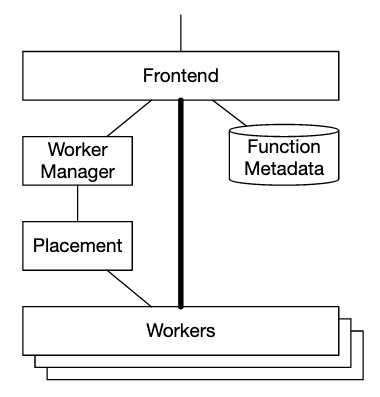
\includegraphics[width=0.35\textwidth]{images/serverless_architecture.png}
	\caption{Serverless Worker-Manager architecture \cite{firecracker}}
	\centering
	\label{fig:arc_serverless}
\end{figure}

\begin{figure*}[!t]
\centering % <-- added
\begin{subfigure}{0.35\textwidth}
  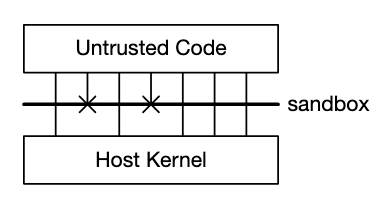
\includegraphics[width=\linewidth]{images/container_architecture.png}
  \caption{Container based Serverless architecture \cite{firecracker}}
  \label{fig:container_serverless}
\end{subfigure} \hfil% <-- added
\begin{subfigure}{0.35\textwidth}
  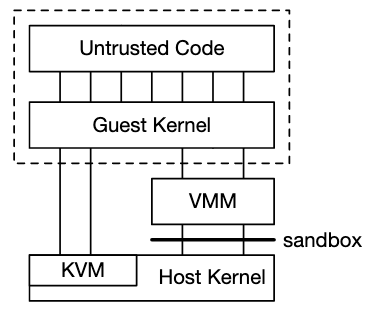
\includegraphics[width=\linewidth]{images/VM_architecture.png}
  \caption{VM based Serverless Architecture \cite{firecracker}}
  \label{fig:human_memory}
\end{subfigure} \hfil% <-- added

\caption{Serverless Architecture}
\label{fig:memory}
\end{figure*}

\subsection*{Lightweight Serverless Computing via Unikernel}
The startup delays of VMs or containers create a higher response latency to users and performance overhead. This paper introduces UaaF (Unikernel-as-a-Function) to provide a lightweight approach to serverless computing that offers a low startup latency to execute functions and a communication model for better inter-functions interactions \cite{tan2020unikernel}. The existing serverless frameworks install all the libraries by an application at startup in every sandbox. As a result, the application finds a high-level redundancy in the memory footprint and high latency in loading libraries. Around 2ms-800ms is needed to load the runtime library when a lambda invocation occurs for the first time, and 80\% of the startup latency is the library installation time \cite{verma2015google}. To avoid a cold start, the authors abstract fine-grained functions from codes and use these shareable libraries in different unikernels and use a special unikernel named ``session'' as a proxy of a serverless application. It holds the sequence of library function invocations and represents the serverless application in the task scheduler. As a result, a session can be executed more quickly. Moreover, UaaF installs separate stacks for different sessions within the virtual address space; therefore, the only copy of library functions need to be stored in the memory that decreases memory repetition across the serverless application shown in \reffig{fig:uaaf_abstraction}.
\begin{figure*}[!t]
\centering % <-- added

\begin{subfigure}{0.56\textwidth}
  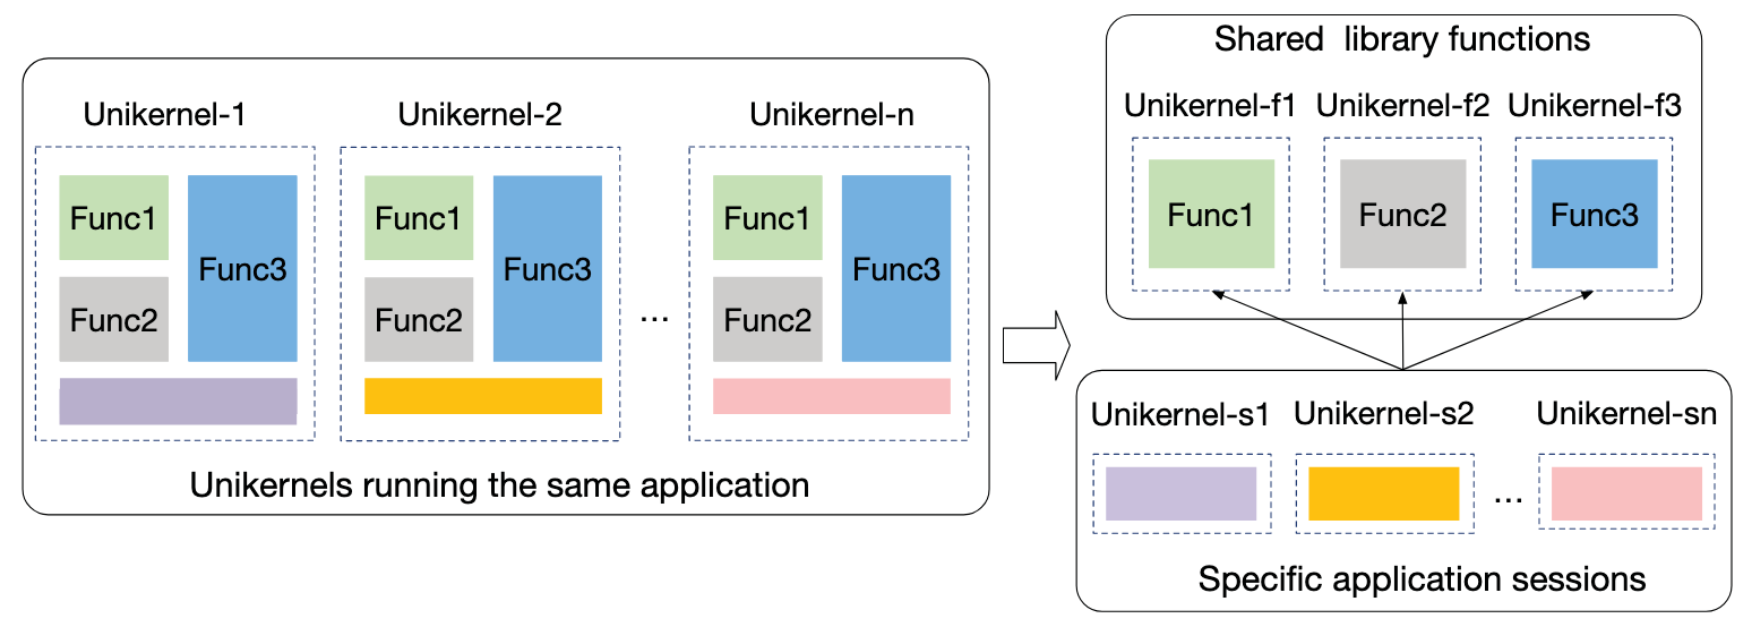
\includegraphics[width=\linewidth]{images/uaaf_abstraction.png}
  \caption{Functions are abstracted form applications and shared by multiple tasks in UaaF}
  \label{fig:uaaf_abstraction}
\end{subfigure} \hfil% <-- added
\begin{subfigure}{0.42\textwidth}
  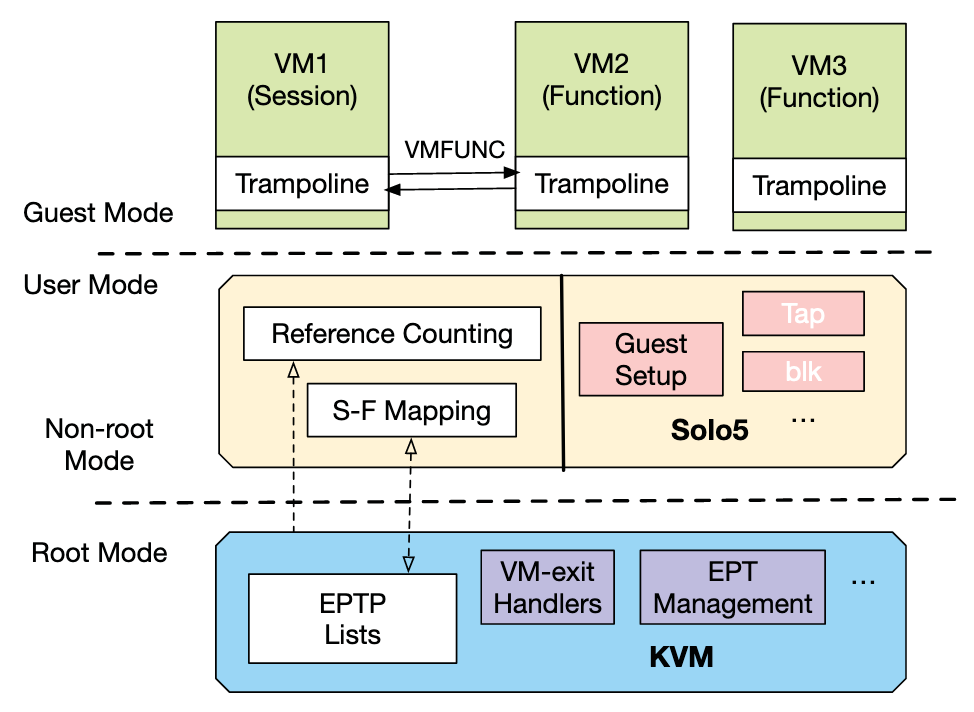
\includegraphics[width=\linewidth]{images/uaaf_architecture.png}
  \caption{The architecture of UaaF}
  \label{fig:uaaf_architecture}
\end{subfigure} \hfil% <-- added
\caption{Unikernel-as-a-Function \cite{tan2020unikernel}}
\label{fig:uaaf}
\end{figure*}
Here is the architecture of UaaF shown in \reffig{fig:uaaf_architecture}. The white modules are proposed by the authors and rests exist in original KVM \cite{kvm} and Solo5 \cite{solo5}. An EPTP (Extend Page Table Pointer) list is a special memory page in the KVM kernel space that has at most 512 EPTP entries pointing to the EPT of other unikernels. The list stores EPT entries used by the VMFUNC instructions. Each unikernel has a trampoline that is used to handle the remote calls between unikernels. UaaF has two modules in user mode. The session-function (S-F) mapping module maintains the mappings between the session ID and the EPTP ID in a table. The reference counting module stores the number of references to each of the functions. The functions that are not referenced, are destroyed by the UaaF.
\begin{figure*}[!b]
\centering % <-- added

\begin{subfigure}{0.34\textwidth}
  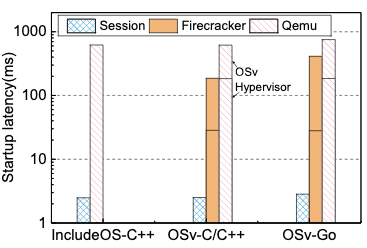
\includegraphics[width=\linewidth]{images/uaaf_start_lat.png}
  \caption{The startup latency of sessions and functions in UaaF}
  \label{fig:uaaf_start_lat}
\end{subfigure} \hfil% <-- added
\begin{subfigure}{0.31\textwidth}
  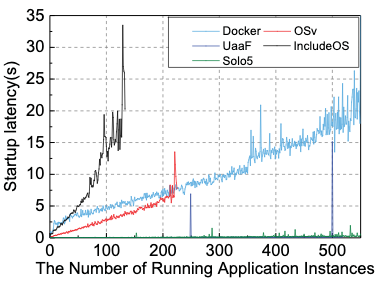
\includegraphics[width=\linewidth]{images/uaaf_start_lat_multiple.png}
  \caption{The startup latency varies with the number of application instances}
  \label{fig:uaaf_startvsmulti}
\end{subfigure} \hfil% <-- added
\begin{subfigure}{0.33\textwidth}
  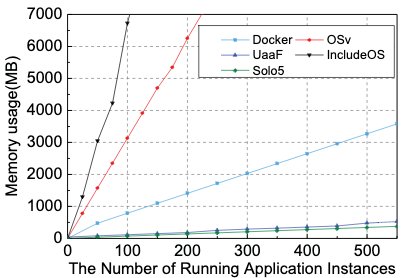
\includegraphics[width=\linewidth]{images/uaaf_multiple_memory.png}
  \caption{The memory usage of differentfunctions and containers}
  \label{fig:uaaf_memoryvsmultiple}
\end{subfigure} \hfil% <-- added
\caption{The performance of UaaF \cite{tan2020unikernel}}
\label{fig:uaaf_performance}
\end{figure*}
\reffig{fig:uaaf_performance} shows the performance of UaaF. \reffig{fig:uaaf_start_lat} shows the startup latency of sessions and functions in UaaF. As UaaF preloaded the functions in memory, the front-end sessions can be started instantly, and UaaF can also limit the application's startup latency below 3ms, which is faster than Firecracker and other traditional unikernels. \reffig{fig:uaaf_startvsmulti} shows the startup latency varies with the number of application instances. As each instance consisted of one session function, and multiple library functions were shared among all instances in UaaF, it can scale large instances similar to Solo5. \reffig{fig:uaaf_memoryvsmultiple} describes the memory usage of different-functions and containers. As we know, IncludeOS, Docker and OSv do not support instances to share execution environments. So, their memory increases linearly with the increasing number of instances. On the other hand, UaaF provides similar memory usage to Solo5 since all library functions were shared.

\todo{Saidur: needs to add limitations}


% \begin{figure}[!ht]
% 	\centering
% 	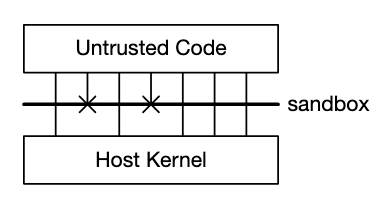
\includegraphics[width=0.5\textwidth]{images/container_architecture.png}
% 	\caption{}
% 	\centering
% 	\label{fig:container_serverless}
% \end{figure}

% \subsection*{VM based serverless}

% \begin{figure}[!ht]
% 	\centering
% 	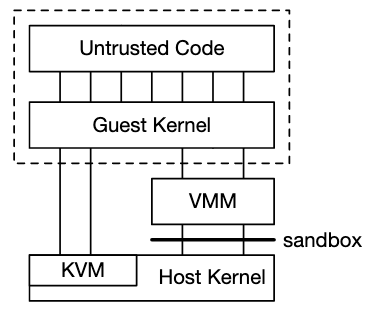
\includegraphics[width=0.5\textwidth]{images/VM_architecture.png}
% 	\caption{VM based Serverless Architecture \cite{firecracker}}
% 	\centering
% 	\label{fig:vm_serverless}
% \end{figure}





\section*{Evaluation}
\label{sec:evaluation}

\subsection*{Serverless Computing Performance}
% \todo{added by Saidur: Jerad please follow the article https://ieeexplore.ieee.org/document/9183650}
\subsubsection*{Fast Boot}
\subsubsection*{Communications}
\subsubsection*{Security}
\subsection*{Container Performance}

\subsection*{VM Performance}

\section*{Discussion}
\label{sec:discussion}

\bibliographystyle{plain}
\bibliography{references/saidur,references/jerad}





%-------------------------------------------------------------------------------

\end{document}

%-------------------------------------------------------------------------------
% SNIPPETS
%-------------------------------------------------------------------------------

%\begin{figure}[!ht]
%	\centering
%	\includegraphics[width=0.8\textwidth]{file_name}
%	\caption{}
%	\centering
%	\label{label:file_name}
%\end{figure}

%\begin{figure}[!ht]
%	\centering
%	\includegraphics[width=0.8\textwidth]{graph}
%	\caption{Blood pressure ranges and associated level of hypertension (American Heart Association, 2013).}
%	\centering
%	\label{label:graph}
%\end{figure}

%\begin{wrapfigure}{r}{0.30\textwidth}
%	\vspace{-40pt}
%	\begin{center}
%		\includegraphics[width=0.29\textwidth]{file_name}
%	\end{center}
%	\vspace{-20pt}
%	\caption{}
%	\label{label:file_name}
%\end{wrapfigure}

%\begin{wrapfigure}{r}{0.45\textwidth}
%	\begin{center}
%		\includegraphics[width=0.29\textwidth]{manometer}
%	\end{center}
%	\caption{Aneroid sphygmomanometer with stethoscope (Medicalexpo, 2012).}
%	\label{label:manometer}
%\end{wrapfigure}

%\begin{table}[!ht]\footnotesize
%	\centering
%	\begin{tabular}{cccccc}
%	\toprule
%	\multicolumn{2}{c} {Pearson's correlation test} & \multicolumn{4}{c} {Independent t-test} \\
%	\midrule	
%	\multicolumn{2}{c} {Gender} & \multicolumn{2}{c} {Activity level} & \multicolumn{2}{c} {Gender} \\
%	\midrule
%	Males & Females & 1st level & 6th level & Males & Females \\
%	\midrule
%	\multicolumn{2}{c} {BMI vs. SP} & \multicolumn{2}{c} {Systolic pressure} & \multicolumn{2}{c} {Systolic Pressure} \\
%	\multicolumn{2}{c} {BMI vs. DP} & \multicolumn{2}{c} {Diastolic pressure} & \multicolumn{2}{c} {Diastolic pressure} \\
%	\multicolumn{2}{c} {BMI vs. MAP} & \multicolumn{2}{c} {MAP} & \multicolumn{2}{c} {MAP} \\
%	\multicolumn{2}{c} {W:H ratio vs. SP} & \multicolumn{2}{c} {BMI} & \multicolumn{2}{c} {BMI} \\
%	\multicolumn{2}{c} {W:H ratio vs. DP} & \multicolumn{2}{c} {W:H ratio} & \multicolumn{2}{c} {W:H ratio} \\
%	\multicolumn{2}{c} {W:H ratio vs. MAP} & \multicolumn{2}{c} {\% Body fat} & \multicolumn{2}{c} {\% Body fat} \\
%	\multicolumn{2}{c} {} & \multicolumn{2}{c} {Height} & \multicolumn{2}{c} {Height} \\
%	\multicolumn{2}{c} {} & \multicolumn{2}{c} {Weight} & \multicolumn{2}{c} {Weight} \\
%	\multicolumn{2}{c} {} & \multicolumn{2}{c} {Heart rate} & \multicolumn{2}{c} {Heart rate} \\
%	\bottomrule
%	\end{tabular}
%	\caption{Parameters that were analysed and related statistical test performed for current study. BMI - body mass index; SP - systolic pressure; DP - diastolic pressure; MAP - mean arterial pressure; W:H ratio - waist to hip ratio.}
%	\label{label:tests}
%\end{table}